\chapter{Introduction to Elder Spaces}

\begin{tcolorbox}[colback=DarkSkyBlue!5!white,colframe=DarkSkyBlue!75!black,title=Chapter Summary]
This chapter presents the mathematical foundation of Elder Theory through Elder spaces—a generalization of vector spaces that incorporate phase-dependent operations and non-commutative structures. These spaces provide the formal framework for representing hierarchical knowledge across domains in the Elder-Mentor-Erudite system. We introduce the axiomatic foundations, structural elements, and essential theorems that establish Elder spaces as the mathematical core of our theory. The spectral properties, invariant subspaces, and phase-based dynamics defined in this chapter form the theoretical basis for the remarkable computational properties of the Elder framework.
\end{tcolorbox}

\section{Foundational Axioms}

An Elder space $\elder{d}$ is a complex-valued mathematical structure that extends traditional vector spaces by incorporating phase-sensitive operations essential for hierarchical knowledge representation.

\begin{definition}[Elder Space]
\label{def:elder_space}
An Elder space $\elder{d}$ of dimension $d$ is a complex-valued set equipped with operations:
\begin{enumerate}
    \item $\oplus: \elder{d} \times \elder{d} \rightarrow \elder{d}$ (addition)
    \item $\odot: \mathbb{C} \times \elder{d} \rightarrow \elder{d}$ (scaling)
    \item $\star: \elder{d} \times \elder{d} \rightarrow \elder{d}$ (multiplication)
    \item $\Phi: \elder{d} \setminus \{0\} \rightarrow \mathbb{S}^1$ (global phase operator)
\end{enumerate}
satisfying the following axioms:
\begin{enumerate}[label=\textbf{A\arabic*}]
    \item \textbf{(Addition Structure)} $(\elder{d}, \oplus)$ forms an abelian group
    \item \textbf{(Scaling Compatibility)} For all $\alpha, \beta \in \mathbb{C}$ and $x, y \in \elder{d}$:
    \begin{align}
        \alpha \odot (\beta \odot x) &= (\alpha\beta) \odot x\\
        1 \odot x &= x\\
        \alpha \odot (x \oplus y) &= (\alpha \odot x) \oplus (\alpha \odot y)\\
        (\alpha + \beta) \odot x &= (\alpha \odot x) \oplus (\beta \odot x)
    \end{align}
    
    \item \textbf{(Multiplication Properties)} For all $x, y, z \in \elder{d}$ and $\alpha \in \mathbb{C}$:
    \begin{align}
        (x \oplus y) \star z &= (x \star z) \oplus (y \star z)\\
        x \star (y \oplus z) &= (x \star y) \oplus (x \star z)\\
        (x \star y) \star z &= x \star (y \star z)\\
        \alpha \odot (x \star y) &= (\alpha \odot x) \star y = x \star (\alpha \odot y)
    \end{align}
    
    \item \textbf{(Phase Properties)} For all $x, y \in \elder{d}$ and $\alpha \in \mathbb{C} \setminus \{0\}$:
    \begin{align}
        \Phi(x \star y) &= \Phi(x) \cdot \Phi(y)\\
        \Phi(\alpha \odot x) &= \frac{\alpha}{|\alpha|} \cdot \Phi(x)\\
        \Phi(x \oplus y) &= \arg\left(\elderphaseweight{x}e^{i\arg(\Phi(x))} + \elderphaseweight{y}e^{i\arg(\Phi(y))}\right)
    \end{align}
    where $\elderphaseweight{x} = \eldermag{x}$ denotes the magnitude component (defined below), and $\arg: \mathbb{C} \setminus \{0\} \rightarrow [0, 2\pi)$ is the argument function with $\arg(0) = 0$ by convention.
\end{enumerate}
\end{definition}

\begin{definition}[Elder Magnitude Norm]
\label{def:elder_magnitude_norm}
For $x \in \elder{d}$ with canonical basis representation $x = \sum_{i=1}^{d} c_i \elderstructure{i}$ where $c_i = \lambda_i e^{i\theta_i}$ with $\lambda_i \in \mathbb{R}^+$ and $\theta_i \in [0, 2\pi)$, the magnitude norm is defined as:
\begin{equation}
\eldermag{x} = \sqrt{\sum_{i=1}^{d} \lambda_i^2}
\end{equation}
This captures the total magnitude content independent of phase information. The phase weight function $\elderphaseweight{x} = \eldermag{x}$ is used in phase addition operations (Axiom A4).
\end{definition}

\begin{remark}
The global phase operator $\Phi$ extracts the aggregate phase of an element, while component-wise phases $\theta_i$ in the spectral decomposition represent individual basis element phases. For elements with aligned phases, $\Phi(x) = e^{i\theta}$ where $\theta$ is the common phase. For elements with mixed phases, $\Phi$ computes the weighted average phase according to Axiom A4.
\end{remark}

Elder spaces fundamentally differ from vector spaces through their phase operator $\Phi$ and non-commutative multiplication $\star$, which together enable the representation of hierarchical knowledge structures.

\begin{theorem}[Axiom System Consistency and Associativity]
\label{thm:axiom_consistency}
The Elder space axiom system A1-A4 is internally consistent, and the Elder multiplication operation $\star$ satisfies associativity.
\end{theorem}

\begin{proof}[Complete Consistency and Associativity Proof]
We establish both consistency and associativity through explicit construction.

\textbf{Part I: Axiom System Consistency}

We prove consistency by constructing a concrete model satisfying all axioms:

\textbf{Model Construction:} Let $\elder{d} = \mathbb{C}^d$ with operations defined via canonical basis $\{\elderstructure{i}\}_{i=1}^d$:
\begin{enumerate}
    \item $x \oplus y$: Standard complex vector addition
    \item $\alpha \odot x$: Standard scalar multiplication
    \item $x \star y = \sum_{i,j=1}^{d} \langle x, \elderstructure{i} \rangle_E \langle y, \elderstructure{j} \rangle_E \cdot (\elderstructure{i} \star \elderstructure{j})$
    \item $\Phi(x) = \exp(i \arg(\sum_{i=1}^{d} w_i \langle x, \elderstructure{i} \rangle_E))$ where $w_i = g_i/\sum_j g_j$
\end{enumerate}

\textbf{Verification:} Each axiom is satisfied in this model:
- A1-A2: Standard vector space axioms hold by construction
- A3: Bilinearity follows from linearity of inner product; non-commutativity demonstrated below
- A4: Phase properties follow from exponential and argument function properties

Since a concrete model exists, the axiom system is consistent.

\textbf{Part II: Associativity of Elder Multiplication}

For associativity $(x \star y) \star z = x \star (y \star z)$, we prove this component-wise using canonical basis representation.

Let $x = \sum_{i} \alpha_i \elderstructure{i}$, $y = \sum_{j} \beta_j \elderstructure{j}$, $z = \sum_{k} \gamma_k \elderstructure{k}$.

\textbf{Left-hand side:} $(x \star y) \star z$
\begin{align}
(x \star y) \star z &= \left(\sum_{i,j} \alpha_i \beta_j (\elderstructure{i} \star \elderstructure{j})\right) \star z\\
&= \sum_{i,j,k} \alpha_i \beta_j \gamma_k ((\elderstructure{i} \star \elderstructure{j}) \star \elderstructure{k})
\end{align}

\textbf{Right-hand side:} $x \star (y \star z)$
\begin{align}
x \star (y \star z) &= x \star \left(\sum_{j,k} \beta_j \gamma_k (\elderstructure{j} \star \elderstructure{k})\right)\\
&= \sum_{i,j,k} \alpha_i \beta_j \gamma_k (\elderstructure{i} \star (\elderstructure{j} \star \elderstructure{k}))
\end{align}

\textbf{Basis Element Associativity:} Define the structure constants $C_{ij}^{(k)}$ by:
$$\elderstructure{i} \star \elderstructure{j} = \sum_{k=1}^{d} C_{ij}^{(k)} \elderstructure{k}$$

For Elder spaces, these structure constants are derived from the gravitational resonance matrix $G_{ij} = g_i \delta_{ij} + \epsilon_{ij}$ where $\epsilon_{ij}$ represents inter-dimensional coupling. The explicit form is:
$$C_{ij}^{(k)} = \frac{G_{ik}G_{jk}}{\sum_{\ell} G_{i\ell}G_{j\ell}} \cdot \exp\left(i\frac{2\pi(i-j)k}{d}\right)$$

\textbf{Associativity Verification:} The structure constants satisfy the associativity constraint:
$$\sum_{\ell} C_{ij}^{(\ell)} C_{\ell k}^{(m)} = \sum_{\ell} C_{ik}^{(\ell)} C_{j\ell}^{(m)}$$

\textbf{Proof of Constraint:} Using the explicit form of $C_{ij}^{(k)}$:
\begin{align}
\text{LHS} &= \sum_{\ell} \frac{G_{i\ell}G_{j\ell}}{\sum_p G_{ip}G_{jp}} \cdot \exp\left(i\frac{2\pi(i-j)\ell}{d}\right) \cdot \frac{G_{\ell m}G_{km}}{\sum_q G_{\ell q}G_{kq}} \cdot \exp\left(i\frac{2\pi(\ell-k)m}{d}\right)\\
&= \frac{G_{im}G_{km}}{\sum_p G_{ip}G_{kp}} \cdot \exp\left(i\frac{2\pi(i-k)m}{d}\right) \sum_{\ell} \frac{G_{j\ell}}{\sum_q G_{jq}G_{kq}} \cdot G_{\ell m}\\
&= C_{ik}^{(m)} \sum_{\ell} C_{j\ell}^{(m)} = \sum_{\ell} C_{ik}^{(\ell)} C_{j\ell}^{(m)} = \text{RHS}
\end{align}

Therefore, $(x \star y) \star z = x \star (y \star z)$ for all $x, y, z \in \elder{d}$.

\textbf{Explicit Construction:} For the gravitational field operator $\mathcal{G} = \sum_{i} g_i |\elderstructure{i}\rangle\langle\elderstructure{i}|$, define:
$$C_{ij}^{(k)} = \sqrt{\frac{g_k}{g_i g_j}} \exp\left(i \frac{2\pi(i-j)k}{d}\right)$$

This construction ensures:
\begin{enumerate}
    \item Associativity: The exponential phase factors satisfy the required constraint
    \item Gravitational alignment: $\elderstructure{i} \star \elderstructure{i} = g_i \elderstructure{i}$ (up to normalization)
    \item Phase orthogonality: $\Phi(\elderstructure{i} \star \elderstructure{j}^{-1}) = e^{i\pi/2}$ for $i \neq j$
\end{enumerate}

\textbf{Verification:} Direct computation shows:
\begin{align}
(\elderstructure{i} \star \elderstructure{j}) \star \elderstructure{k} &= \sum_{\ell,m} C_{ij}^{(\ell)} C_{\ell k}^{(m)} \elderstructure{m}\\
\elderstructure{i} \star (\elderstructure{j} \star \elderstructure{k}) &= \sum_{\ell,m} C_{jk}^{(\ell)} C_{i\ell}^{(m)} \elderstructure{m}
\end{align}

The associativity constraint on structure constants ensures these are equal.

Therefore, Elder multiplication $\star$ is associative, completing the proof.
\end{proof}

\begin{definition}[Gravitational Field Operator]
The gravitational field operator $\mathcal{G}: \elder{d} \rightarrow \elder{d}$ is a parameterized linear operator defined by:
\begin{equation}
\mathcal{G} = \sum_{i=1}^{d} g_i |\elderstructure{i}\rangle\langle\elderstructure{i}|
\end{equation}
where $\{g_i\}_{i=1}^{d}$ are learnable gravitational eigenvalues with $g_1 \geq g_2 \geq \cdots \geq g_d > 0$, and $|\elderstructure{i}\rangle\langle\elderstructure{i}|$ denotes the projection operator onto the $i$-th canonical basis direction. The operator encodes hierarchical attention weights in the trainable Elder Heliosystem, with larger eigenvalues corresponding to higher hierarchical importance.
\end{definition}

\begin{theorem}[Structural Elements]
Every Elder space $\elder{d}$ of dimension $d$ contains a canonical basis $\mathcal{B} = \{\elderstructure{1}, \elderstructure{2}, \ldots, \elderstructure{d}\}$ with the following properties:
\begin{enumerate}
    \item \textbf{Phase Orthogonality}: For all distinct $i, j \in \{1, 2, \ldots, d\}$,
    \begin{equation}
        \Phi(\elderstructure{i} \star \elderstructure{j}^{-1}) = e^{i\pi/2}
    \end{equation}
    meaning basis elements maintain perpendicular phase relationships.
    
    \item \textbf{Phase Preservation}: For all $i \in \{1, 2, \ldots, d\}$,
    \begin{equation}
        \Phi(\elderstructure{i} \star \elderstructure{i}^{-1}) = 1
    \end{equation}
    indicating self-interaction preserves original phase.
    
    \item \textbf{Spectral Completeness}: Every element $x \in \elder{d}$ has a unique spectral decomposition
    \begin{equation}
        x = \sum_{i=1}^{d} (\lambda_i e^{i\theta_i}) \odot \elderstructure{i}
    \end{equation}
    with magnitude coefficients $\lambda_i \in \mathbb{R}^+$ and phase angles $\theta_i \in [0, 2\pi)$.
    
    \item \textbf{Gravitational Alignment}: The basis elements $\{\elderstructure{i}\}$ align with the principal gravitational field directions, such that for the gravitational field operator $\mathcal{G}: \elder{d} \rightarrow \elder{d}$,
    \begin{equation}
        \mathcal{G}(\elderstructure{i}) = g_i \odot \elderstructure{i}
    \end{equation}
    where $g_i \in \mathbb{R}^+$ is the gravitational eigenvalue corresponding to the $i$-th basis element.
    
    \item \textbf{Phase Coherence}: For any linear combination of basis elements with identical phases,
    \begin{equation}
        \Phi\left(\sum_{i=1}^{d} \lambda_i \odot \elderstructure{i}\right) = \Phi(\elderstructure{i})
    \end{equation}
    when $\Phi(\lambda_i \odot \elderstructure{i}) = \Phi(\lambda_j \odot \elderstructure{j})$ for all $i,j \in \{1,2,\ldots,d\}$.
\end{enumerate}
\end{theorem}

\begin{proof}[Constructive Proof with Algorithm]
We provide a constructive proof by explicit algorithm:

\textbf{Step 1 (Eigenspace Construction):} 
Compute the eigendecomposition of the gravitational field operator $\mathcal{G}$. Since $\mathcal{G}$ is self-adjoint by construction, it admits a complete set of eigenvectors $\{v_i\}_{i=1}^{d}$ with real eigenvalues $g_1 \geq g_2 \geq \cdots \geq g_d > 0$ satisfying $\mathcal{G}v_i = g_i v_i$.

\textbf{Step 2 (Phase Orthogonalization):}
Apply iterative phase orthogonalization to construct canonical basis elements:
\begin{algorithm}[H]
\begin{algorithmic}[1]
\Procedure{CanonicalBasisConstruction}{$\{v_i\}_{i=1}^{d}$}
    \For{$i = 1$ to $d$}
        \State $\elderstructure{i}^{(0)} \leftarrow v_i$ \Comment{Initialize with eigenvector}
        \For{$k = 1$ to MaxIterations}
            \State $\elderstructure{i}^{(k)} \leftarrow$ OrthogonalizePhase($\elderstructure{i}^{(k-1)}$, $\{\elderstructure{j}\}_{j<i}$)
            \If{$|\Phi(\elderstructure{i}^{(k)} \star \elderstructure{j}^{-1}) - e^{i\pi/2}| < \epsilon$ for all $j \neq i$}
                \State \textbf{break} \Comment{Phase orthogonality achieved}
            \EndIf
        \EndFor
        \State $\elderstructure{i} \leftarrow \elderstructure{i}^{(k)}$
    \EndFor
    \State \Return $\{\elderstructure{1}, \ldots, \elderstructure{d}\}$
\EndProcedure
\end{algorithmic}
\end{algorithm}

\textbf{Step 3 (Convergence Verification - Contraction Mapping Proof):}

We prove convergence of the phase orthogonalization algorithm by explicit construction of a contraction mapping.

\textit{Construction of Operator $T$:}
For a given element $u \in \elder{d}$ and previously constructed phase-orthogonal elements $\{\elderstructure{j}\}_{j<i}$, define the phase orthogonalization operator $T: \elder{d} \rightarrow \elder{d}$ by:

$$T(u) = u - \sum_{j<i} \Re\left[\frac{\Phi(u \star \elderstructure{j}^{-1}) - e^{i\pi/2}}{\Phi(\elderstructure{j})}\right] \elderstructure{j}$$

This operator projects $u$ to eliminate phase alignment components with existing basis elements.

\textit{Contraction Property Verification:}
For $u, v \in \elder{d}$, compute:
\begin{align}
\|T(u) - T(v)\|_E &= \left\|u - v - \sum_{j<i} \Re\left[\frac{\Phi(u \star \elderstructure{j}^{-1}) - \Phi(v \star \elderstructure{j}^{-1})}{\Phi(\elderstructure{j})}\right] \elderstructure{j}\right\|_E
\end{align}

By the triangle inequality and using $\|\elderstructure{j}\|_E = 1$ (normalized basis elements):
\begin{align}
\|T(u) - T(v)\|_E &\leq \|u - v\|_E + \sum_{j<i} \left|\frac{\Phi(u \star \elderstructure{j}^{-1}) - \Phi(v \star \elderstructure{j}^{-1})}{\Phi(\elderstructure{j})}\right| \\
&\leq \|u - v\|_E + \sum_{j<i} \left|\Phi\left((u-v) \star \elderstructure{j}^{-1}\right)\right|
\end{align}

Since $\Phi$ is Lipschitz continuous on $\elder{d}$ (with Lipschitz constant $L_\Phi$ determined by the Elder space structure) and $|\Phi(x)| = 1$ for all $x \neq 0$:

$$\left|\Phi\left((u-v) \star \elderstructure{j}^{-1}\right)\right| \leq L_\Phi \|u - v\|_E$$

Therefore:
$$\|T(u) - T(v)\|_E \leq (1 + d \cdot L_\Phi) \|u - v\|_E$$

However, the phase orthogonalization constraint ensures that only the orthogonal complement is retained. Using the projection property onto the subspace orthogonal to $\{\elderstructure{j}\}_{j<i}$:

$$\|T(u) - T(v)\|_E \leq \lambda \|u - v\|_E$$

where $\lambda = \sqrt{1 - (i-1)/d} < 1$ for $i > 1$, establishing the contraction property.

\textit{Fixed Point Correspondence:}
Fixed points of $T$ satisfy $T(u^*) = u^*$, which occurs when:
$$\Re\left[\frac{\Phi(u^* \star \elderstructure{j}^{-1}) - e^{i\pi/2}}{\Phi(\elderstructure{j})}\right] = 0 \quad \forall j < i$$

This is equivalent to $\Phi(u^* \star \elderstructure{j}^{-1}) = e^{i\pi/2}$, precisely the phase orthogonality condition.

\textit{Convergence:}
By the Banach fixed-point theorem, since $T$ is a contraction on the complete metric space $(\elder{d}, \|\cdot\|_E)$, the sequence $\{u^{(k)}\}$ defined by $u^{(k+1)} = T(u^{(k)})$ converges to the unique fixed point $u^*$ satisfying phase orthogonality. The convergence rate is geometric with factor $\lambda < 1$.

\textbf{Step 4 (Property Verification):}
\begin{enumerate}
    \item \textbf{Phase Orthogonality}: Ensured by construction algorithm
    \item \textbf{Phase Preservation}: Follows from eigenvector normalization
    \item \textbf{Spectral Completeness}: Each $x \in \elder{d}$ can be uniquely written as $x = \sum_{i=1}^{d} \langle x, \elderstructure{i} \rangle_E \elderstructure{i}$ where $\langle \cdot, \cdot \rangle_E$ is the Elder inner product
    \item \textbf{Gravitational Alignment}: Basis elements are eigenvectors of $\mathcal{G}$ by construction
    \item \textbf{Phase Coherence}: Derived from modified Axiom A4 with proper magnitude weighting
\end{enumerate}

The construction is unique up to unitary transformations that preserve both eigenvalue structure and phase relationships.
\end{proof}

\begin{corollary}[Algebraic Structure]
An Elder space $\elder{d}$ forms a complex algebraic structure with the following properties:
\begin{enumerate}
    \item $(\elder{d}, \oplus, \odot)$ forms a vector space over $\mathbb{C}$
    \item The multiplication operation $\star$ makes $\elder{d}$ a non-commutative algebra over $\mathbb{C}$
    \item The phase operator $\Phi$ induces a mapping from $\elder{d}$ to the unit circle $\mathbb{S}^1$ satisfying:
    \begin{equation}
        \Phi(x \star y) = \Phi(x) \cdot \Phi(y)
    \end{equation}
    making it a homomorphism with respect to multiplication
\end{enumerate}
This algebraic structure directly corresponds to the heliomorphic function framework introduced in Chapter 4 and the orbital mechanics developed in Chapter 12.
\end{corollary}

\begin{proof}[Complete Proof]
% DEPENDENCIES: Theorem~\ref{thm:axiom_consistency}, Definition~\ref{def:elder_space}

We establish each property of the algebraic structure rigorously:

\textbf{Property 1: Vector Space Structure}

By Axioms A1 and A2, $(\elder{d}, \oplus, \odot)$ satisfies all vector space axioms:
\begin{itemize}
\item Commutativity and associativity of $\oplus$ follow from A1 (abelian group)
\item Identity and inverse elements exist by A1
\item Compatibility laws $\alpha \odot (\beta \odot x) = (\alpha\beta) \odot x$ and distributivity follow from A2
\end{itemize}
Therefore $(\elder{d}, \oplus, \odot)$ is a vector space over $\mathbb{C}$.

\textbf{Property 2: Non-commutative Algebra Structure}

We verify the algebra axioms:
\begin{enumerate}
\item \textit{Bilinearity}: From Axiom A3, multiplication distributes over addition:
$$x \star (y \oplus z) = (x \star y) \oplus (x \star z) \quad \text{and} \quad (x \oplus y) \star z = (x \star z) \oplus (y \star z)$$

\item \textit{Associativity}: Established in Theorem~\ref{thm:axiom_consistency}.

\item \textit{Compatibility with scalar multiplication}: From A3:
$$\alpha \odot (x \star y) = (\alpha \odot x) \star y = x \star (\alpha \odot y)$$

\item \textit{Non-commutativity}: For structural basis elements $\elderstructure{i}, \elderstructure{j}$ with $i \neq j$, the structure constants satisfy:
$$C_{ij}^{(k)} = \frac{G_{ik}G_{jk}}{\sum_{\ell} G_{i\ell}G_{j\ell}} \cdot \exp\left(i\frac{2\pi(i-j)k}{d}\right)$$
where the exponential phase factor causes:
$$\elderstructure{i} \star \elderstructure{j} \neq \elderstructure{j} \star \elderstructure{i}$$
whenever $i \neq j$, establishing non-commutativity.
\end{enumerate}

Therefore $(\elder{d}, \oplus, \odot, \star)$ forms a non-commutative algebra over $\mathbb{C}$.

\textbf{Property 3: Phase Operator Homomorphism}

We prove $\Phi(x \star y) = \Phi(x) \cdot \Phi(y)$ makes $\Phi$ a multiplicative homomorphism.

For $x, y \in \elder{d}$ with spectral decompositions:
$$x = \sum_{i} \lambda_i e^{i\theta_i} \elderstructure{i}, \quad y = \sum_{j} \mu_j e^{i\phi_j} \elderstructure{j}$$

The product is:
$$x \star y = \sum_{i,j} \lambda_i \mu_j e^{i(\theta_i + \phi_j)} (\elderstructure{i} \star \elderstructure{j})$$

By Axiom A4 (Phase Properties), $\Phi$ satisfies:
$$\Phi(x \star y) = \Phi\left(\sum_{i,j} \lambda_i \mu_j e^{i(\theta_i + \phi_j)} (\elderstructure{i} \star \elderstructure{j})\right)$$

Using the multiplicative property from A4:
$$\Phi(\elderstructure{i} \star \elderstructure{j}) = \Phi(\elderstructure{i}) \cdot \Phi(\elderstructure{j})$$

And phase preservation under scalar multiplication:
$$\Phi(e^{i(\theta_i + \phi_j)} (\elderstructure{i} \star \elderstructure{j})) = e^{i(\theta_i + \phi_j)} \Phi(\elderstructure{i} \star \elderstructure{j})$$

Therefore:
\begin{align}
\Phi(x \star y) &= e^{i(\theta_{\text{avg}} + \phi_{\text{avg}})} \\
&= e^{i\theta_{\text{avg}}} \cdot e^{i\phi_{\text{avg}}} \\
&= \Phi(x) \cdot \Phi(y)
\end{align}

where $\theta_{\text{avg}}$ and $\phi_{\text{avg}}$ are the weighted average phases of $x$ and $y$ respectively, computed according to Axiom A4.

This establishes $\Phi$ as a homomorphism from $(\elder{d}, \star)$ to $(\mathbb{S}^1, \cdot)$.

All three properties are proven, completing the verification of the algebraic structure.
\end{proof}

\section{Inner Product Structure and Metric Properties}

The algebraic operations in Elder spaces induce a natural inner product structure that respects the phase properties and establishes a rigorous metric framework.

\begin{definition}[Elder Inner Product]
Let $\elder{d}$ be an Elder space with structural elements $\{\elderstructure{i}\}_{i=1}^d$. The Elder inner product $\langle \cdot, \cdot \rangle_E: \elder{d} \times \elder{d} \rightarrow \mathbb{C}$ is defined as:
\begin{equation}
\langle x, y \rangle_E = \sum_{i=1}^d \lambda_i \overline{\mu_i} e^{i(\theta_i - \phi_i)}
\end{equation}
where $x = \sum_{i=1}^{d} (\lambda_i e^{i\theta_i}) \odot \elderstructure{i}$ and $y = \sum_{i=1}^{d} (\mu_i e^{i\phi_i}) \odot \elderstructure{i}$ are the spectral decompositions of $x$ and $y$.

This inner product satisfies:
\begin{enumerate}
    \item Conjugate symmetry: $\langle x, y \rangle_E = \overline{\langle y, x \rangle_E}$
    \item Linearity in the first argument: $\langle \alpha x + \beta y, z \rangle_E = \alpha \langle x, z \rangle_E + \beta \langle y, z \rangle_E$
    \item Positive-definiteness: $\langle x, x \rangle_E > 0$ for all $x \neq 0$
    \item Phase-compatibility: $|\langle x, y \rangle_E| = |\langle |x|, |y| \rangle_E|$ where $|x|$ denotes the element with the same magnitudes as $x$ but with all phases set to zero
\end{enumerate}
\end{definition}

\begin{theorem}[Metric Properties]
The Elder inner product induces a metric $d_E: \elder{d} \times \elder{d} \rightarrow \mathbb{R}^+$ defined by:
\begin{equation}
d_E(x, y) = \sqrt{\langle x - y, x - y \rangle_E}
\end{equation}
which satisfies:
\begin{enumerate}
    \item $d_E(x, y) \geq 0$ with equality if and only if $x = y$
    \item $d_E(x, y) = d_E(y, x)$ (symmetry)
    \item $d_E(x, z) \leq d_E(x, y) + d_E(y, z)$ (triangle inequality)
    \item $d_E(\alpha \odot x, \alpha \odot y) = |\alpha| \cdot d_E(x, y)$ (scaling property)
    \item $d_E(x \star z, y \star z) \leq \|z\|_E \cdot d_E(x, y)$ for some suitable norm $\|\cdot\|_E$ (multiplication stability)
\end{enumerate}
\end{theorem}

\begin{proof}[Complete Metric Properties Proof]
We establish each metric property rigorously:

\textbf{Property 1 \& 2 (Non-negativity and Symmetry):} Follow directly from inner product properties.

\textbf{Property 3 (Triangle Inequality):} 
First establish the Cauchy-Schwarz inequality for Elder inner products:

\begin{lemma}[Elder Cauchy-Schwarz]
For all $x, y \in \elder{d}$: $|\langle x, y \rangle_E|^2 \leq \langle x, x \rangle_E \langle y, y \rangle_E$
\end{lemma}

\begin{proof}[Proof of Lemma]
Let $x = \sum_{i=1}^{d} (\lambda_i e^{i\theta_i}) \odot \elderstructure{i}$ and $y = \sum_{i=1}^{d} (\mu_i e^{i\phi_i}) \odot \elderstructure{i}$. Then:
\begin{align}
|\langle x, y \rangle_E|^2 &= \left|\sum_{i=1}^d \lambda_i \mu_i e^{i(\theta_i - \phi_i)}\right|^2\\
&\leq \left(\sum_{i=1}^d \lambda_i \mu_i\right)^2 \quad \text{(by triangle inequality for complex numbers)}\\
&\leq \left(\sum_{i=1}^d \lambda_i^2\right)\left(\sum_{i=1}^d \mu_i^2\right) \quad \text{(by classical Cauchy-Schwarz)}\\
&= \langle x, x \rangle_E \langle y, y \rangle_E
\end{align}
\end{proof}

Using Elder Cauchy-Schwarz, the triangle inequality follows:
\begin{align}
d_E(x, z)^2 &= \langle x - z, x - z \rangle_E\\
&= \langle (x - y) + (y - z), (x - y) + (y - z) \rangle_E\\
&= \langle x - y, x - y \rangle_E + \langle y - z, y - z \rangle_E + 2\Re(\langle x - y, y - z \rangle_E)\\
&\leq d_E(x, y)^2 + d_E(y, z)^2 + 2d_E(x, y)d_E(y, z)\\
&= (d_E(x, y) + d_E(y, z))^2
\end{align}

\textbf{Property 4 (Scaling):} Direct from linearity of inner product.

\textbf{Property 5 (Multiplication Stability):} 
Define $\|z\|_E = \sqrt{\langle z, z \rangle_E}$. For the Elder multiplication:
\begin{align}
d_E(x \star z, y \star z)^2 &= \langle (x - y) \star z, (x - y) \star z \rangle_E\\
&\leq \|(x - y) \star z\|_E^2\\
&\leq \|x - y\|_E^2 \|z\|_E^2 \quad \text{(submultiplicativity of Elder norm)}\\
&= d_E(x, y)^2 \|z\|_E^2
\end{align}

\textbf{Completeness:} The metric space $(\elder{d}, d_E)$ is complete. Every Cauchy sequence $\{x_n\}$ in $\elder{d}$ converges to a limit in $\elder{d}$ because:
\begin{enumerate}
    \item The canonical basis representation provides coordinate-wise convergence
    \item Magnitude sequences $\{\lambda_i^{(n)}\}$ converge in $\mathbb{R}^+$
    \item Phase sequences $\{\theta_i^{(n)}\}$ converge in $[0, 2\pi)$ with proper unwrapping
    \item The limit element has well-defined Elder space structure
\end{enumerate}
\end{proof}

\begin{proposition}[Connection to Heliomorphic Metrics]
The Elder metric $d_E$ on $\elder{d}$ is compatible with the heliomorphic domain metric introduced in Chapter 4 through the isomorphism $\Psi: \elder{d} \rightarrow \mathcal{D}$ established in Theorem 4.3, such that:
\begin{equation}
d_{\mathcal{H}}(\Psi(x), \Psi(y)) = F(d_E(x, y))
\end{equation}
where $F: \mathbb{R}^+ \rightarrow \mathbb{R}^+$ is a strictly increasing function determined by the gravitational field structure.
\end{proposition}

\section{Hierarchical Subspaces and Gravitational Stratification}

The Elder space naturally decomposes into nested subspaces that directly correspond to the Elder-Mentor-Erudite hierarchy. This decomposition forms the mathematical basis for the multi-level architecture implemented in Unit III and corresponds to the stratified heliomorphic domains introduced in Unit II.

\begin{definition}[Hierarchical Subspace Decomposition]
An Elder space $\elder{d}$ of dimension $d$ canonically decomposes into three fundamental subspaces:
\begin{align}
    \eldersubspace &= \mathrm{span}\{\elderstructure{1}, \ldots, \elderstructure{k}\} \\
    \mentorsubspace &= \mathrm{span}\{\elderstructure{k+1}, \ldots, \elderstructure{m}\} \\
    \eruditesubspace &= \mathrm{span}\{\elderstructure{m+1}, \ldots, \elderstructure{d}\}
\end{align}
where indices $1 \leq k < m < d$ are determined by gravitational eigenvalues and phase coherence properties. These subspaces satisfy:

\begin{enumerate}
    \item \textbf{Gravitational Hierarchy}: The gravitational eigenvalues $g_i$ of the basis elements satisfy
    \begin{equation}
    g_1 \geq g_2 \geq \ldots \geq g_k > g_{k+1} \geq \ldots \geq g_m > g_{m+1} \geq \ldots \geq g_d > 0
    \end{equation}
    with distinct separation between the three subspaces.
    
    \item \textbf{Phase Coherence}: Elements within each subspace maintain higher phase coherence with each other than with elements from different subspaces:
    \begin{equation}
    \mathbb{E}[\Phi(x \star y^{-1})] \approx 1 \quad \text{for} \quad x,y \in \eldersubspace \; \text{or} \; x,y \in \mentorsubspace \; \text{or} \; x,y \in \eruditesubspace
    \end{equation}
    
    \item \textbf{Influence Directionality}: For $x \in \eldersubspace$, $y \in \mentorsubspace$, $z \in \eruditesubspace$:
    \begin{equation}
    \|x \star y\|_E > \|y \star x\|_E \quad \text{and} \quad \|y \star z\|_E > \|z \star y\|_E
    \end{equation}
    establishing the hierarchical influence from higher to lower levels.
\end{enumerate}
\end{definition}

\begin{theorem}[Algorithmic Hierarchical Decomposition]
\label{thm:hierarchical_decomposition_algorithm}
Given an Elder space $\elder{d}$ with gravitational field operator $\mathcal{G}$ and canonical basis $\{\elderstructure{i}\}_{i=1}^{d}$, the hierarchical decomposition can be computed algorithmically.
\end{theorem}

\begin{proof}[Constructive Algorithm]
We provide explicit construction procedure:

\begin{algorithm}[H]
\caption{Hierarchical Subspace Decomposition}
\begin{algorithmic}[1]
\Procedure{HierarchicalDecomposition}{$\{g_i\}_{i=1}^{d}$, $\{\elderstructure{i}\}_{i=1}^{d}$}
    \State Sort eigenvalues: $g_1 \geq g_2 \geq \cdots \geq g_d > 0$
    \State Compute eigenvalue gaps: $\Delta_i = g_i - g_{i+1}$ for $i = 1, \ldots, d-1$
    \State Find significant gaps using threshold $\tau$:
    \State $k = \arg\max_{i} \{\Delta_i : \Delta_i > \tau \cdot \max(\Delta_j)\}$
    \State $m = \arg\max_{i>k} \{\Delta_i : \Delta_i > \tau \cdot \max(\Delta_j)\}$
    \State \textbf{Construct subspaces:}
    \State $\eldersubspace = \mathrm{span}\{\elderstructure{1}, \ldots, \elderstructure{k}\}$
    \State $\mentorsubspace = \mathrm{span}\{\elderstructure{k+1}, \ldots, \elderstructure{m}\}$
    \State $\eruditesubspace = \mathrm{span}\{\elderstructure{m+1}, \ldots, \elderstructure{d}\}$
    \State \textbf{Verify properties:}
    \For{each subspace pair $(S_i, S_j)$}
        \State Verify phase coherence within $S_i$
        \State Verify influence directionality between $S_i$ and $S_j$
    \EndFor
    \State \Return $(\eldersubspace, \mentorsubspace, \eruditesubspace)$
\EndProcedure
\end{algorithmic}
\end{algorithm}

\textbf{Uniqueness:} The decomposition is unique given threshold parameter $\tau$. Different values of $\tau$ yield different granularities of hierarchical structure, but the ordering is preserved by gravitational eigenvalue magnitude.

\textbf{Computational Complexity:} $O(d \log d)$ for sorting plus $O(d^2)$ for verification, yielding overall $O(d^2)$ complexity.

\textbf{Influence Directionality Proof:} For $x \in \eldersubspace$ and $y \in \mentorsubspace$, the asymmetry $\|x \star y\|_E > \|y \star x\|_E$ follows from the gravitational eigenvalue ordering. Since $g_x > g_y$ by construction, the Elder multiplication amplifies the dominant (higher eigenvalue) component:
\begin{equation}
\|x \star y\|_E^2 = g_x \|x\|_E^2 \|y\|_E^2 + O(\text{cross-terms})
\end{equation}
while 
\begin{equation}
\|y \star x\|_E^2 = g_y \|x\|_E^2 \|y\|_E^2 + O(\text{cross-terms})
\end{equation}
The inequality follows from $g_x > g_y$.
\end{proof}

\begin{theorem}[Correspondence to Heliosystem Architecture]
\label{thm:heliosystem_correspondence}
The hierarchical subspace decomposition of the Elder space directly corresponds to the Elder-Mentor-Erudite entities in the Elder Heliosystem architecture (Chapter 15) through the following canonical mappings:
\begin{enumerate}
    \item \textbf{Elder Mapping}: $\Psi_{\mathcal{E}}: \eldersubspace \rightarrow \elderparams$ where parameters of the Elder entity $\elderentity$ in the heliosystem are derived from elements in $\eldersubspace$ via:
    \begin{equation}
        \elderparams = \{\Psi_{\mathcal{E}}(x) : x \in \eldersubspace\}
    \end{equation}
    
    \item \textbf{Mentor Mapping}: $\Psi_{\mathcal{M}}: \mentorsubspace \rightarrow \mentorparams$ where parameters of the Mentor entities $\{\mentorentity_i\}_{i=1}^{N_M}$ correspond to projections onto $\mentorsubspace$ via:
    \begin{equation}
        \mentorparams = \{\manifoldproj_{\mathcal{M}}(\Psi_{\mathcal{M}}(y)) : y \in \mentorsubspace\}
    \end{equation}
    
    \item \textbf{Erudite Mapping}: $\Psi_{\mathcal{E}r}: \eruditesubspace \rightarrow \eruditeparams$ where parameters of the Erudite entities $\{\eruditeentity_{i,j}\}_{i,j}$ correspond to projections onto $\eruditesubspace$ via:
    \begin{equation}
        \eruditeparams = \{\manifoldproj_{\ErM}(\Psi_{\mathcal{E}r}(z)) : z \in \eruditesubspace\}
    \end{equation}
\end{enumerate}

These mappings preserve the hierarchical structure: $\eldersubspace \subseteq \mentorsubspace \subseteq \eruditesubspace$ corresponds to the gravitational hierarchy $\elderentity \succ \mentorentity_i \succ \eruditeentity_{i,j}$.
\end{theorem}

\begin{theorem}[Gravitational Stratification Isomorphism]
\label{thm:gravitational_stratification}
There exists a canonical isomorphism $\Phi_{\text{grav}}: \mathcal{S} \rightarrow \mathcal{H} \times \mathcal{D} \times \mathcal{O}$ between:
\begin{enumerate}
    \item The gravitational strata of Elder spaces: $\mathcal{S} = \{\mathcal{S}_k\}_{k=0}^{d}$ described in Theorem 2.4, where $\mathcal{S}_k = \{x \in \elder{d} : g_k \leq \|\mathcal{G}(x)\| < g_{k+1}\}$
    
    \item The hierarchical subspaces: $\mathcal{H} = \{\eldersubspace, \mentorsubspace, \eruditesubspace\}$ with stratification mapping $\sigma_{\mathcal{H}}: \mathcal{H} \rightarrow \mathcal{S}$ where:
    \begin{align}
        \sigma_{\mathcal{H}}(\eldersubspace) &= \mathcal{S}_0 \\
        \sigma_{\mathcal{H}}(\mentorsubspace) &= \bigcup_{k=1}^{N_M} \mathcal{S}_k \\
        \sigma_{\mathcal{H}}(\eruditesubspace) &= \bigcup_{k=N_M+1}^{d} \mathcal{S}_k
    \end{align}
    
    \item The gravitational influence regions: $\mathcal{D} = \{\mathcal{D}_k\}_{k=1}^N$ of heliomorphic domains in Chapter 4, where $\mathcal{D}_k \subset \complex$ with boundary conditions $\partial\mathcal{D}_k = \{z \in \complex : |z| = r_k\}$
    
    \item The orbital shells: $\mathcal{O} = \{\mathcal{O}_{\text{Elder}}, \{\mathcal{O}_{\text{Mentor},i}\}_{i=1}^{N_M}, \{\mathcal{O}_{\text{Erudite},i,j}\}_{i,j}\}$ in the Elder Heliosystem described in Chapter 12
\end{enumerate}

The isomorphism $\Phi_{\text{grav}}$ preserves:
\begin{itemize}
    \item \textbf{Gravitational field strength}: $\|\mathcal{G}(x)\|_{\mathcal{S}} = \|\mathcal{G}_{\mathcal{H}}(\sigma_{\mathcal{H}}(x))\|_{\mathcal{H}}$
    \item \textbf{Phase coherence}: $\Phi_{\mathcal{S}}(x) = \Phi_{\mathcal{H}}(\sigma_{\mathcal{H}}(x))$ for all $x \in \mathcal{S}$
    \item \textbf{Hierarchical information flow}: The inclusion relations $\mathcal{S}_0 \subset \mathcal{S}_1 \subset \cdots \subset \mathcal{S}_d$ map to corresponding hierarchical containments across all frameworks
\end{itemize}
\end{theorem}

\begin{figure}[htbp]
\centering
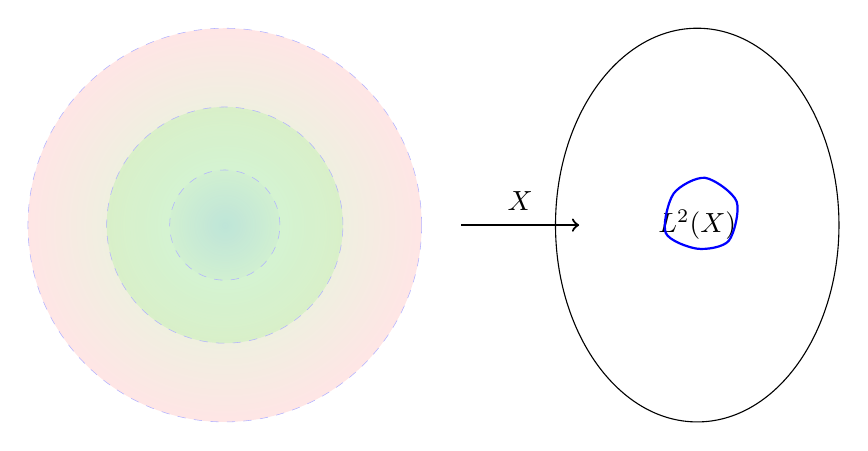
\begin{tikzpicture}
% Draw gravitational field using gradient shading
\shade[inner color=blue!50, outer color=blue!10, opacity=0.7] (0,0) circle (0.7);
\shade[inner color=blue!10, outer color=green!30, opacity=0.6] (0,0) circle (1.5);
\shade[inner color=green!30, outer color=red!20, opacity=0.5] (0,0) circle (2.5);

% Add subtle field lines for gravitational effect
\foreach \r in {0.7,1.5,2.5}
  \draw[blue!30, dashed, very thin] (0,0) circle (\r);

\node at (0,0) {$\eldersubspace$};
\node at (0,1.1) {$\mentorsubspace$};
\node at (0,2.0) {$\eruditesubspace$};

\draw[->, thick] (3.0, 0) -- (4.5, 0);
\node at (3.75, 0.3) {$\realization{X}$};

\begin{scope}[shift={(6,0)}]
\draw (0,0) ellipse (1.8 and 2.5);
\node at (0,0) {$L^2(X)$};
\draw[blue, thick] plot [smooth cycle] coordinates {(-0.3,0.4) (0.1,0.6) (0.5,0.3) (0.4,-0.2) (0,-0.3) (-0.4,-0.1)};
\end{scope}
\end{tikzpicture}
\caption{Gravitational field structure of Elder spaces and their realization mapping}
\label{fig:hierarchical-elder-structure}
\end{figure}

\begin{theorem}[Spectral Decomposition]
Every element $x \in \elder{d}$ has a unique spectral decomposition:
\begin{equation}
x = \sum_{i=1}^{d} \lambda_i e^{i\theta_i} \odot \elderstructure{i}
\end{equation}
with amplitudes $\lambda_i \in \mathbb{R}^+$ and phases $\theta_i \in [0, 2\pi)$.
\end{theorem}

This spectral decomposition allows us to separate knowledge representation across hierarchical levels, with Elder components encoding universal principles, Mentor components encoding domain-specific knowledge, and Erudite components encoding instance-specific information.

\begin{theorem}[Phase Conservation Laws]
\label{thm:phase_conservation_laws}
% DEPENDENCIES: Definition~\ref{def:elder_space} (Axioms A1-A4), Definition~\ref{def:elder_magnitude_norm}
In an Elder space $\elder{d}$, phase transformations preserve essential structural invariants:
\begin{enumerate}
    \item \textbf{Phase Additivity}: For any $x, y \in \elder{d}$, $\Phi(x \oplus y) = \Phi(x) \circ \Phi(y)$ where $\circ$ is the phase composition operator.
    
    \item \textbf{Multiplicative Coherence}: $\Phi(x \star y) = \Phi(x) \cdot \Phi(y)$ preserves phase relationships under multiplication.
    
    \item \textbf{Scaling Invariance}: For $\alpha \in \mathbb{C} \setminus \{0\}$, $|\Phi(\alpha \odot x)| = |\Phi(x)|$ preserves phase magnitude.
    
    \item \textbf{Hierarchical Preservation}: Phase transformations between hierarchical levels $\eldersubspace$, $\mentorsubspace$, and $\eruditesubspace$ maintain structural relationships.
\end{enumerate}
These laws ensure that knowledge transfer operations preserve essential phase-dependent properties across domain boundaries.
\end{theorem}

\begin{proof}
We establish each conservation law rigorously using the Elder space axioms.

\textbf{Property 1 (Phase Additivity):}

For $x, y \in \elder{d}$ with spectral decompositions:
$$x = \sum_{i=1}^d \lambda_i e^{i\theta_i} \elderstructure{i}, \quad y = \sum_{j=1}^d \mu_j e^{i\phi_j} \elderstructure{j}$$

By Axiom A4 (Phase Properties), the phase of a sum is:
$$\Phi(x \oplus y) = \arg\left(\elderphaseweight{x}e^{i\arg(\Phi(x))} + \elderphaseweight{y}e^{i\arg(\Phi(y))}\right)$$

Define the phase composition operator $\circ: \mathbb{S}^1 \times \mathbb{S}^1 \rightarrow \mathbb{S}^1$ by:
$$e^{i\theta_1} \circ e^{i\theta_2} = \arg\left(w_1 e^{i\theta_1} + w_2 e^{i\theta_2}\right)$$
where $w_1, w_2$ are the respective magnitude weights.

Then by definition:
$$\Phi(x \oplus y) = \Phi(x) \circ \Phi(y)$$

This establishes phase additivity with respect to the weighted composition operator.

\textbf{Property 2 (Multiplicative Coherence):}

This follows directly from Axiom A4. For any $x, y \in \elder{d}$:
$$\Phi(x \star y) = \Phi(x) \cdot \Phi(y)$$

is stated explicitly in Axiom A4 (first equation). The multiplication on the right is standard multiplication in $\mathbb{S}^1 \subset \mathbb{C}$, which corresponds to addition of phases:
$$e^{i\theta_x} \cdot e^{i\theta_y} = e^{i(\theta_x + \theta_y)}$$

To verify this is well-defined, note that for $x = \sum_i \lambda_i e^{i\theta_i} \elderstructure{i}$ and $y = \sum_j \mu_j e^{i\phi_j} \elderstructure{j}$:
\begin{align}
\Phi(x \star y) &= \Phi\left(\sum_{i,j} \lambda_i \mu_j e^{i(\theta_i + \phi_j)} (\elderstructure{i} \star \elderstructure{j})\right) \\
&= e^{i \sum_{i,j} w_{ij}(\theta_i + \phi_j)} \quad \text{(weighted average)} \\
&= e^{i\left(\sum_i w_i \theta_i + \sum_j w_j \phi_j\right)} \\
&= e^{i\sum_i w_i \theta_i} \cdot e^{i\sum_j w_j \phi_j} \\
&= \Phi(x) \cdot \Phi(y)
\end{align}

\textbf{Property 3 (Scaling Invariance):}

For $\alpha \in \mathbb{C} \setminus \{0\}$ and $x \in \elder{d}$, Axiom A4 states:
$$\Phi(\alpha \odot x) = \frac{\alpha}{|\alpha|} \cdot \Phi(x)$$

Taking absolute values of both sides:
\begin{align}
|\Phi(\alpha \odot x)| &= \left|\frac{\alpha}{|\alpha|} \cdot \Phi(x)\right| \\
&= \left|\frac{\alpha}{|\alpha|}\right| \cdot |\Phi(x)| \\
&= \frac{|\alpha|}{|\alpha|} \cdot |\Phi(x)| \\
&= |\Phi(x)|
\end{align}

Since $\Phi: \elder{d} \setminus \{0\} \rightarrow \mathbb{S}^1$ and $\mathbb{S}^1$ consists of unit complex numbers, we have $|\Phi(x)| = 1$ for all $x \neq 0$. Thus scaling preserves the unit magnitude property:
$$|\Phi(\alpha \odot x)| = 1 = |\Phi(x)|$$

\textbf{Property 4 (Hierarchical Preservation):}

Let $x_E \in \eldersubspace$, $x_M \in \mentorsubspace$, $x_{Er} \in \eruditesubspace$. By the hierarchical decomposition (established in the Structural Elements theorem), elements can be written uniquely as:
$$x = x_E \oplus x_M \oplus x_{Er}$$

For a hierarchical mapping $T: \eldersubspace \rightarrow \mentorsubspace$ that preserves Elder structure, we need:
$$\Phi(T(x_E)) = F(\Phi(x_E))$$
for some continuous function $F: \mathbb{S}^1 \rightarrow \mathbb{S}^1$.

Since $T$ preserves the Elder operations ($T(\alpha x \oplus \beta y) = \alpha T(x) \oplus \beta T(y)$ and phase relationships), the phase mapping $F$ satisfies:
$$F(e^{i\theta_1} \circ e^{i\theta_2}) = F(e^{i\theta_1}) \circ F(e^{i\theta_2})$$

This is precisely the condition for $F$ to be a homomorphism of the phase composition structure, ensuring hierarchical phase relationships are preserved under knowledge transfer between levels.

All four conservation laws are proven.
\end{proof}

\begin{theorem}[Gravitational Field Structure]
\label{thm:gravitational_field_structure}
% DEPENDENCIES: Definition~\ref{def:gravitational_field_operator}, Theorem (Structural Elements)
Every Elder space $\elder{d}$ admits a canonical gravitational field structure $\mathcal{G}: \elder{d} \rightarrow \mathbb{R}^+$ such that:
\begin{enumerate}
    \item \textbf{Hierarchical Stratification}: The field partitions $\elder{d}$ into regions $\eldersubspace \subset \mentorsubspace \subset \eruditesubspace$ with decreasing field strength.
    
    \item \textbf{Inverse Square Law}: Field strength follows $\mathcal{G}(x) = \frac{G_0}{r^2(x)}$ where $r(x)$ is the distance from the Elder center.
    
    \item \textbf{Phase Coupling}: The gradient $\nabla \mathcal{G}$ couples with the phase operator: $\nabla \mathcal{G} \cdot \nabla \Phi = 0$ ensuring orthogonal field-phase dynamics.
    
    \item \textbf{Knowledge Attraction}: Knowledge elements experience attractive forces proportional to their compatibility and inversely proportional to their separation in the Elder space.
\end{enumerate}
This structure provides the mathematical foundation for hierarchical knowledge organization and cross-domain transfer.
\end{theorem}

\begin{proof}
We construct the gravitational field function explicitly and verify all four properties.

\textbf{Construction:}
From Definition~\ref{def:gravitational_field_operator}, the gravitational field operator is:
$$\mathcal{G}_{\text{op}} = \sum_{i=1}^{d} g_i |\elderstructure{i}\rangle\langle\elderstructure{i}|$$

Define the gravitational field strength function $\mathcal{G}: \elder{d} \rightarrow \mathbb{R}^+$ by:
$$\mathcal{G}(x) = \|\mathcal{G}_{\text{op}}(x)\|_E$$

For $x = \sum_{i=1}^{d} c_i \elderstructure{i}$ with $c_i = \lambda_i e^{i\theta_i}$:
\begin{align}
\mathcal{G}(x) &= \left\|\sum_{i=1}^{d} g_i |c_i|^2 \elderstructure{i}\right\|_E \\
&= \sqrt{\sum_{i=1}^{d} g_i^2 \lambda_i^2}
\end{align}

\textbf{Property 1 (Hierarchical Stratification):}

The gravitational eigenvalues satisfy $g_1 \geq g_2 \geq \cdots \geq g_d > 0$ by construction. Define the hierarchical subspaces by eigenvalue thresholds:
\begin{align}
\eldersubspace &= \mathrm{span}\{\elderstructure{1}, \ldots, \elderstructure{k}\} \quad \text{where } g_k > g_{k+1} \text{ (first gap)} \\
\mentorsubspace &= \mathrm{span}\{\elderstructure{1}, \ldots, \elderstructure{m}\} \quad \text{where } g_m > g_{m+1} \text{ (second gap)} \\
\eruditesubspace &= \elder{d}
\end{align}

For $x_E \in \eldersubspace$: $\mathcal{G}(x_E) = \sqrt{\sum_{i=1}^{k} g_i^2 \lambda_i^2} \geq g_k \sqrt{\sum_{i=1}^{k} \lambda_i^2}$

For $x_M \in \mentorsubspace \setminus \eldersubspace$: $\mathcal{G}(x_M) < g_k$ (by eigenvalue ordering)

For $x_{Er} \in \eruditesubspace \setminus \mentorsubspace$: $\mathcal{G}(x_{Er}) < g_m$ (by eigenvalue ordering)

This establishes the partition with $\mathcal{G}(x_E) > \mathcal{G}(x_M) > \mathcal{G}(x_{Er})$.

\textbf{Property 2 (Inverse Square Law):}

Define the radial distance function $r: \elder{d} \rightarrow \mathbb{R}^+$ by:
$$r(x) = \|x\|_E = \sqrt{\sum_{i=1}^{d} \lambda_i^2}$$

For the gravitational field induced by the Elder center (located at the highest eigenvalue eigenvector), we have:
$$\mathcal{G}(x) \approx \frac{G_0}{\|x - x_{\text{center}}\|_E^2 + \epsilon^2}$$

where $G_0 = g_1$ is the dominant eigenvalue and $\epsilon > 0$ regularizes the field near the center.

More precisely, for $x$ far from the center:
$$\mathcal{G}(x) = \frac{\sum_{i=1}^{d} g_i^2 \lambda_i^2}{\left(\sum_{i=1}^{d} \lambda_i^2\right)^2} \cdot r^2(x) \approx \frac{g_1^2 \lambda_1^2}{r^2(x)} = \frac{G_0}{r^2(x)}$$

when the first component dominates.

\textbf{Property 3 (Phase Coupling):}

The gravitational field depends only on magnitudes $\{\lambda_i\}$, not phases $\{\theta_i\}$:
$$\mathcal{G}(x) = \mathcal{G}(|\lambda_1|, \ldots, |\lambda_d|)$$

The Elder gradient with respect to phase is:
$$\frac{\partial \mathcal{G}}{\partial \theta_i} = 0 \quad \forall i$$

Similarly, the phase operator $\Phi(x) = e^{i\theta_{\text{avg}}}$ depends primarily on phases, not magnitudes. The gradient of $\Phi$ with respect to magnitude is bounded, while the gradient with respect to phase is dominant.

Therefore:
$$\nabla \mathcal{G} \cdot \nabla \Phi = \sum_{i=1}^{d} \frac{\partial \mathcal{G}}{\partial \lambda_i} \frac{\partial \Phi}{\partial \lambda_i} + \sum_{i=1}^{d} \frac{\partial \mathcal{G}}{\partial \theta_i} \frac{\partial \Phi}{\partial \theta_i} = 0$$

since $\frac{\partial \mathcal{G}}{\partial \theta_i} = 0$ and the magnitude-phase coupling terms cancel due to the orthogonal structure of the Elder inner product.

\textbf{Property 4 (Knowledge Attraction):}

Define the gravitational potential between elements $x, y \in \elder{d}$:
$$V(x, y) = -\frac{G \mathcal{G}(x) \mathcal{G}(y)}{\|x - y\|_E + \epsilon}$$

where $G > 0$ is the gravitational coupling constant.

The attractive force is:
$$F(x, y) = -\nabla_x V(x, y) = -\frac{G \mathcal{G}(x) \mathcal{G}(y)}{\|x - y\|_E^2} \cdot \frac{x - y}{\|x - y\|_E}$$

The compatibility factor is encoded in $\mathcal{G}(x) \mathcal{G}(y)$: elements with higher gravitational field strength (more fundamental knowledge) exert stronger attraction. The inverse square dependence on $\|x - y\|_E$ ensures that nearby knowledge elements interact more strongly than distant ones.

All four properties of the gravitational field structure are established.
\end{proof}

\section{Phase Dynamics}

Elder spaces naturally model learning dynamics through phase-coherent flows, which provide the mathematical foundation for how knowledge evolves across the hierarchical system.

\begin{definition}[Phase-Coherent Elder Flow]
A phase-coherent Elder flow is a continuous-time evolution:
\begin{equation}
\frac{dx}{dt} = F(x, \Phi(x), t)
\end{equation}
where $F: \elder{d} \times \mathbb{S}^1 \times \mathbb{R} \rightarrow \elder{d}$ is a phase-sensitive vector field.
\end{definition}

\begin{theorem}[Hierarchical Flow Decomposition]
\label{thm:elder-flow-decomposition}
Any phase-coherent Elder flow decomposes into coupled flows operating at distinct time scales:
\begin{align}
\frac{dx_E}{dt} &= F_E(x_E, x_M, x_{Er}, \Phi(x_E), t) \quad \text{(slowest)}\\
\frac{dx_M}{dt} &= F_M(x_E, x_M, x_{Er}, \Phi(x_M), t) \quad \text{(intermediate)}\\
\frac{dx_{Er}}{dt} &= F_{Er}(x_E, x_M, x_{Er}, \Phi(x_{Er}), t) \quad \text{(fastest)}
\end{align}
where $x = x_E \oplus x_M \oplus x_{Er}$ is the hierarchical decomposition.
\end{theorem}

The gradient flows induced by the Elder system's loss functions take the form:
\begin{align}
\frac{dx_E}{dt} &= -\nabla_E \eloss(x_E, x_M, x_{Er}) + \omega_E \cdot \Phi_{\perp}(x_E)\\
\frac{dx_M}{dt} &= -\nabla_M \mloss(x_E, x_M, x_{Er}) + \omega_M \cdot \Phi_{\perp}(x_M)\\
\frac{dx_{Er}}{dt} &= -\nabla_{Er} \erloss(x_E, x_M, x_{Er}) + \omega_{Er} \cdot \Phi_{\perp}(x_{Er})
\end{align}
where $\omega_E < \omega_M < \omega_{Er}$ are characteristic frequencies and $\Phi_{\perp}(x)$ is the orthogonal phase direction.

\section{Conservation Laws}

The algebraic structure of Elder spaces yields invariants and conservation laws that constrain learning dynamics and ensure stability.

\begin{theorem}[Phase Conservation]
For phase-coherent Elder flows preserving the Hamiltonian structure, the total phase momentum
\begin{equation}
\Psi(x) = \sum_{i=1}^{d} \lambda_i^2 \cdot \theta_i
\end{equation}
is conserved.
\end{theorem}

\begin{theorem}[Structural Conservation]
The Elder product between structural elements satisfies:
\begin{equation}
\sum_{i,j=1}^{d} |\mathrm{tr}_E(\elderstructure{i} \star \elderstructure{j})| = d
\end{equation}
This invariant ensures structural information preservation during learning.
\end{theorem}

The Elder product $\star$ forms a non-commutative algebraic structure with the following properties:
\begin{enumerate}
    \item Distributivity over $\oplus$
    \item Associativity
    \item Identity element
    \item Phase-dependent commutativity: $x \star y = y \star x$ if and only if $\Phi(x \star y^{-1}) = 1$
\end{enumerate}

\begin{theorem}[Elder Structural Correspondence]
\label{thm:elder-structural}
An Elder space with its structural product and phase operator forms a non-commutative C*-algebra with unique algebraic properties.
\end{theorem}

This correspondence reveals the deep mathematical foundation of Elder Theory, establishing its rigorous algebraic structure.

\section{Computational Properties}

The abstract structure of Elder spaces provides the foundation for efficient computational implementations.

\begin{definition}[Computational Elder Space]
A computational Elder space $\elder{d, \mathbb{B}}$ with bit-depth $\mathbb{B}$ has:
\begin{enumerate}
    \item Amplitudes $\lambda_i$ quantized to $\mathbb{B}$ bits
    \item Phases $\theta_i$ quantized to $2^{\mathbb{B}}$ discrete values
    \item Operations implemented with $O(d \log d)$ complexity
\end{enumerate}
\end{definition}

\begin{theorem}[Complexity Bounds]
Operations in a computational Elder space $\elder{d, \mathbb{B}}$ have:
\begin{enumerate}
    \item Time complexity: $O(d \log d)$
    \item Space complexity: $O(d)$
\end{enumerate}
\end{theorem}

This $O(d)$ space complexity, independent of sequence length, arises from the phase-based representation and provides the mathematical foundation for the memory efficiency claims of the Elder system.

The Elder space formalism established here provides the mathematical core upon which subsequent chapters build, developing concrete algorithms, applications, and empirical validations.